\subsection{Desenvolver Suíte de Testes Automatizados}

A suíte de testes automatizados possui a responsabilidade de garantir o correto funcionamento da integração entre os sistemas envolvidos, ou seja prover um meio onde possa ser testado o Webservice do GSAN e o Middleware juntamente com o Asterisk, neste cenário foram utilizados recursos do JUnit para criação dos cenários de teste, execução dos testes e identificação de falhas, quanto recursos do \textit{framework} Asterisk-Java para estabelecer a conexão com o Asterisk, criando e monitorando chamadas telefônicas com parametrização dinâmica.   

Os testes criados utilizando o \textit{framework} JUnit, podem ser executados a qualquer momento, seja manualmente pela própria IDE de desenvolvimento quanto de forma automatizada por algum ambiente de integração contínua, que realiza a inspeção de qualidade disparando a execução dos testes, visando garantir o correto comportamento do sistema na construção de uma entrega ou \textit{release}.

A suíte de teste é composta por classes constantes com a parametrização necessária para configuração da conexão com o Asterisk, classe de serviço para realizar o \textit{Login}, \textit{Logoff} e iniciar uma chamada telefônica, conta também com uma classe utilitária que permite registrar ouvintes em chamadas telefônicas gerada. Dessa forma é possível estabelecer uma conexão com o Asterisk, realizar chamadas telefônica para contexto locais da ferramenta e acompanhar o comportamento apresentado.

Cada classe de teste deve implementar uma interface do \textit{framework} Asterisk-Java chamada \textit{PropertyChangeListener} e posteriormente ser registrada como \textit{Listener} em uma classe da suíte chamada \textit{SuiteAsteriskListener}, que atua como um ouvinte de modificações que ocorrem nos canais, tais canais representam as chamadas telefônicas existentes na ferramenta. 
A classe de teste deve ser configurada para sempre antes de executar um teste realiza primeiro o \textit{Login} na ferramenta Asterisk e ao final da execução do teste efetuar o \textit{Logoff}, somente após o \textit{Login} é possível iniciar a simulação das chamadas para os contextos de testes, abaixo está demonstrado o funcionamento da suíte de teste automatizado integrado a uma classe de teste conforme a figura \ref{figura:diagramaSeq2Via};

\begin{figure}[H]
	\centering
	\caption{Diagrama de sequência utilizando a suíte de teste.}
	\label{figura:diagramaSeq2Via}
	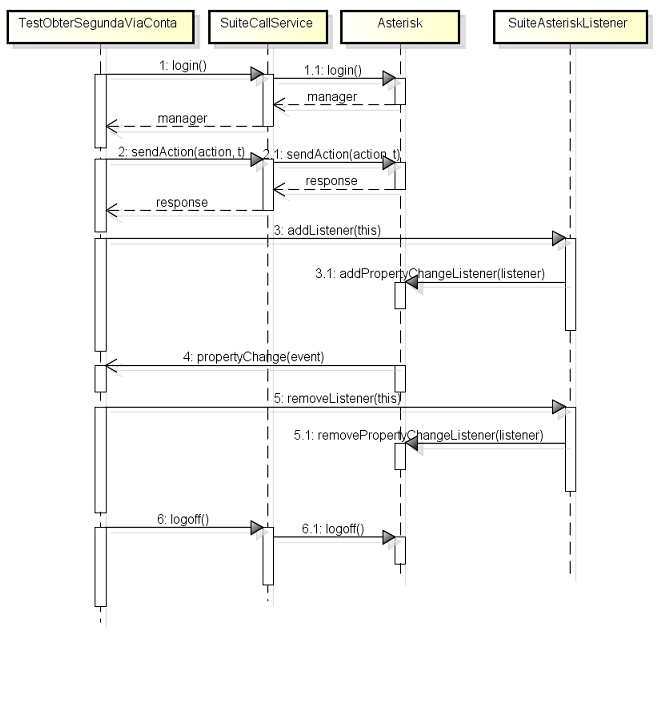
\includegraphics{figuras/diagramaSequenciaObter2Via.png}
	\legend {\fontsize{10}{12}\selectfont {Fonte: Autoria Própria}.}
\end{figure}

O diagrama demostrado na figura \ref{figura:diagramaSeq2Via} ilustra o funcionamento da classe de teste para o serviço Obter 2ª via de conta, trabalhando em conjunto com a suíte de teste, inicialmente é realizado o \textit{Login} com a ferramenta Asterisk, para obter o objeto \textit{manager} que permite a comunicação com o Asterisk, logo em seguida é criada a chamada telefônica e passada como \textit{action} juntamente com um tempo limite de esperar para o método \textit{sendAction}, tal ação é destinada ao Asterisk para estabelecer a criação do canal de comunicação, após a confirmação do retorno a classe de teste chama o método \textit{addListener} com intuito de ser registrada como ouvinte das mudanças que ocorrem nos canais abertos, a suíte de teste faz o registro do \textit{listener} junto ao Asterisk,
quando o Asterisk identifica mudança no canal dispara uma notificação através do método \textit{propertyChange} com detalhes do evento para a classe ouvinte registrada, com essa informação a classe de teste pode identificar o comportamento apresentado pelo canal, ao final a classe de teste remove o registro de ouvinte e realiza o \textit{Logoff}, chamando respectivamente os métodos \textit{removeListener} e \textit{logoff}.


Durante a execução de um cenário de teste, é necessário monitorar o comportamento da chamada ou canal internamento na ferramente Asterisk,
afim de validar o retorno obtido pela requisição e posteriormente evidenciar a ocorrência do comportamento esperado ou de falhas. Com isso se faz necessário habilitar a conexão remota na ferramenta Asterisk. O arquivo \textit{/etc/asterisk/manager.conf} contém as propriedades necessárias para serem configuradas, abaixo é demostrado a configuração realizada para execução dos testes automatizados;
\\
\hspace{10 mm}\textit{[general]} 			\hspace{10 mm} $\triangleright$ Contexto geral de conexão.\\
\hspace{10 mm}\textit{enabled=yes}  		\hspace{10 mm} $\triangleright$ Habilitar a conexão remota.\\
\hspace{10 mm}\textit{port=5038}  			\hspace{10 mm} $\triangleright$ Define a porta.\\
\hspace{10 mm}\textit{displayconnects=yes}  \hspace{10 mm} $\triangleright$ Define a exibição das conexões no console.\\
\hspace{10 mm}\textit{permit=0.0.0.0/0.0.0.0} \hspace{10 mm} $\triangleright$ Define o endereço IP que será aceito.\\

Abaixo segue o exemplo de configuração para adição de um novo usuário para conexão remota;
\\
\hspace{10 mm}\textit{[manager]} 	\hspace{10 mm} $\triangleright$ Nome do novo usuário.\\
\hspace{10 mm}\textit{secret=pa55w0rd} \hspace{10 mm} $\triangleright$ Senha do novo usuário \\
\hspace{10 mm}\textit{read=system,call,log,verbose,command,agent}  \hspace{10 mm} $\triangleright$ Define as permissões de leitura.\\
\hspace{10 mm}\textit{write=system,call,log,verbose,command,agent}  \hspace{10 mm} $\triangleright$ Define as permissões de escrita.\\
\hspace{10 mm}\textit{permit=0.0.0.0/0.0.0.0} \hspace{10 mm} $\triangleright$ Define o endereço IP que será aceito \\


A distribuição Disc-OS por padrão possui uma configuração de \textit{firewall} bastante restritiva por questões de segurança, para que não ocorra rejeição nas solicitações realizadas ao Asterisk, será para fins de testes desabilitada as regras do firewall, utilizando o seguinte comando \textit{/etc/init.d/iptables stop}.
 
A suíte de testes contém a implementação dos testes de integração para os três serviços automatizados que são obter 2º via de conta, informar falta de água e solicitar restabelecimento da ligação de água, além de testes unitários para verificação da rotina de enviar e-mail e checagem da disponibilidade do Webservice.


